\documentclass[10pt]{article}
\usepackage[italian]{babel}
\usepackage{amsmath,amsfonts,amssymb,mathtools, ulem, booktabs,subcaption}
\usepackage[utf8x]{inputenc}
\usepackage[margin=1.0in]{geometry}

\title{Fondamenti di Matematica per Informatica: Schema Esercizi}
\author{Aymane Chabbaki}
\date{II semestre 2018/2019}
\begin{document}
	\maketitle
	\tableofcontents
	\newpage
	
  \section{Principio di Induzione}
	\subsection{Cosa specificare durante lo sviluppo di un esercizio}
	\begin{itemize}
	\item
	\textsc{Base dell'induzione}
	\item
	\textsc{Passo induttivo}
	\item
	\textsc{Ipotesi induttiva}
	\end{itemize}
	
	\subsection{Esercizio 1}
	Si dimostri per induzione su $n \!\in\! \mathbb{N}$ che $\forall \, n \!\geq\! 1$ $P(n) := \displaystyle{\left(\sum_{k=0}^n \frac{5^k}{4^k} = \frac{5^{n+1}}{4^n} - 4 \right)}$
	\\ \textsc{Soluzione:}
	\begin{itemize}
	\item
	Osserviamo che vale $n=1$ (\textbf{base dell'induzione}):
	\begin{equation}
	\begin{split}
	\displaystyle{\frac{5^0}{4^0} + \frac{5^1}{4^1}} &= \displaystyle{\frac{5^{1+1}}{4^1} - 4} \\
	\displaystyle{1 + \frac{5}{4}} &= \displaystyle{\frac{25}{4} - 4}\\
	\displaystyle{\frac{9}{4}} &= \displaystyle{\frac{9}{4}}
	\notag
	\end{split}
	\end{equation}
	\item
	Dunque $P(0)$  vera.
	\item
	$n \implies n + 1$ (\textbf{passo induttivo}) con $n \!\geq\! 1$.
	\item
	Assumo che l'ugualianza: $\displaystyle{\sum_{k=0}^n \frac{5^k}{4^k} = \frac{5^{n+1}}{4^n} - 4}$ (\textbf{ipotesi induttiva}) sia vera.
	\item
	Devo dimostare che: $\displaystyle{\sum_{k=0}^{n+1} \frac{5^k}{4^k} = \frac{5^{(n+1)+1}}{4^{n+1}} - 4}$
	\item
	Vale:
	\begin{equation}
	\begin{split}
	\displaystyle{\sum_{k=0}^{n+1} \frac{5^k}{4^k}} &= \displaystyle{\left(\sum_{k=0}^{n} \frac{5^k}{4^k}\right) + \frac{5^{n+1}}{4^{n+1}}} \\
	\textrm{\small{(\textbf{ipotesi induttiva})}} \mapsto &= \displaystyle{\left(\frac{5^{n+1}}{4^{n}}\right) + \frac{5^{n+1}}{4^{n+1}}} \\
	&= \displaystyle{\frac{4 \cdot 5^{n+1} + 5^{n+1}}{4^{n+1}} -4} \\		
	&= \displaystyle{\frac{5 \cdot 5^{n+1}}{4^{n+1}}-4} \\		
	&= \displaystyle{\frac{5^{(n+1)+1}}{4^{n+1}}-4}
	\notag
	\end{split}
	\end{equation}
	\item
	Dunque, visto che $\displaystyle{\sum_{k=0}^{n+1} \frac{5^k}{4^k} =\frac{5^{(n+1)+1}}{4^{n+1}}-4}$, abbiamo dimostrato l'ugualianza.
	\end{itemize}
	\newpage
	
	\subsection{Esercizio 2}
	Si dimostri per induzione su $n \!\in\! \mathbb{N}$ che $\forall \, n \geq 2$ $P(n) := \displaystyle{\left(\sum_{k=1}^n \frac{5}{6^k} = 1 - \frac{1}{6^n} \right)}$
	\\ \textsc{Soluzione:}
	\begin{itemize}
	\item
	Osserviamo che vale $n=2$ (\textbf{base dell'induzione}):
	\begin{equation}
	\begin{split}
	\displaystyle{\sum_{k=1}^2 \frac{5}{6^k}} &= \displaystyle{1 - \frac{1}{6^2}} \\
	\displaystyle{\frac{5}{6} + \frac{5}{6^2}} &= \displaystyle{1 - \frac{1}{36}} \\
	\displaystyle{\frac{6*5 + 5}{36}} &= \displaystyle{\frac{36 - 1}{36}} \\ 
	\displaystyle{\frac{35}{36}} &= \displaystyle{\frac{35}{36}}
	\notag
	\end{split}
	\end{equation}
	\item
	$P(2)$ è vera.
	\item
	\textbf{1° modo:}
	\begin{itemize}
	\item
	$n \!\geq\! 2$, $n \implies n+1$
	\item
	Assumiamo $P(n)$ sia verificata per qualche $n \geq 2$ (\textbf{ipotesi induttiva}).
	\item
	Dimostriamo che $P(n+1)$ è vera, ovvero $\displaystyle{\sum_{k=1}^{n+1} \frac{5}{6^k} = 1 - \frac{1}{6^{n+1}}}$ è vera (\textbf{passo induttivo}).
	\item
	Vale:
	\begin{equation}
	\begin{split}
	\sum_{k=1}^{n+1} \frac{5}{6^k} &= \left(\sum_{k=1}^{n} \frac{5}{6^k}\right) + \frac{5}{6^{n+1}} \\
	\textrm{\small{(\textbf{ipotesi induttiva})}} \mapsto &= \left(1 - \frac{1}{6^n} \right) + \frac{5}{6^{n+1}} \\
	&= 1 - \frac{1}{6^n} + \frac{5}{6^{n+1}} \\
	&= 1 - \left(\frac{1}{6^n} - \frac{5}{6^{n+1}}\right) \\
	&= 1 - \left(\frac{6-5}{6^{n+1}} \right) \\
	&= 1 - \frac{1}{6^{n+1}} 
	\notag
	\end{split}
	\end{equation}
	\item
	Dunque, visto che $\displaystyle{\sum_{k=1}^{n+1} \frac{5}{6^k} = 1 - \frac{1}{6^{n+1}}}$, abbiamo dimostrato l'ugualianza.
	\end{itemize}
	
	\item
	\textbf{2° modo:}
	\begin{itemize}
	\item
	$n \!\geq\! 2$, $n \implies n+1$ e assumiamo che valga $\displaystyle{\sum_{k=1}^{n} \frac{5}{6^k} = 1 - \frac{1}{6^{n}}}$ per qualche $n \geq 2$ (\textbf{ipotesi induttiva}).
	\item
	Devo dimostrare che vale: $\displaystyle{\sum_{k=1}^{n+1} \frac{5}{6^k} = 1 - \frac{1}{6^{n+1}}}$
	\item
	Vale:
	\begin{equation}
	\begin{split}
	\sum_{k=1}^{n+1} \frac{5}{6^k} &= 1 - \frac{1}{6^{n+1}}\Longleftrightarrow \\
	  \left(\sum_{k=1}^{n} \frac{5}{6^k}\right) + \frac{5}{6^{n+1}} &= 1 - \frac{1}{6^{n+1}}\Longleftrightarrow \\
	 1 - \frac{1}{6^n} + \frac{5}{6^{n+1}} &= 1 - \frac{1}{6^{n+1}}\Longleftrightarrow \\
	 \frac{1}{6^{n+1}} + \frac{5}{6^{n+1}} &= \frac{1}{6^{n}}\Longleftrightarrow \\
	 \frac{6}{6^{n+1}} &= \frac{1}{6^{n}}\Longleftrightarrow \\
	 \frac{1}{6^{n}} &= \frac{1}{6^{n}}
	 \notag
	\end{split}
	\end{equation}
	\end{itemize}
	\item
	Osserviamo che l'ultima equazione è un'\textbf{identità} (sempre vera) e dunque, visto che le operazioni sono delle \textbf{succesioni di equivalenze}, si può affermare che anche la prima uguaglianza è soddisfatta.
	\end{itemize}
	
  \subsection{Esercizio 3}
	Si dimostri per induzione su $n \!\in\! \mathbb{N}$ che $\forall \, n \geq 1$, vale $P(n) := \displaystyle{\left(\sum_{k=0}^n 4 \cdot k \cdot 3^k = 3 + 3^{n+1} (2n-1) \right)}$
	\\ \textsc{Soluzione:}
	\begin{itemize}
	\item
	Osserviamo che vale $n=1$ (\textbf{base dell'induzione}):
	\begin{equation}
	\begin{split}
	\sum_{k=0}^1 4 \cdot k \cdot 3^k &= 3 + 3^{1+1} (2 \cdot 1 -1) \\
	4 \cdot 0 \cdot 3^0 + 4 \cdot 1 \cdot 3^1 &= 3+3^2(2-1) \\
	12 &= 12
	\notag
	\end{split}
	\end{equation}
	\item
	$P(1)$ risulta vera.
	\item
	$n \!\geq\! 1, n \implies n+1$
	\item
	Assumiamo $P(n)$ vera per qualche $n \!\geq\! 1$ (\textbf{ipotesi induttiva}).
	\item
	Dimostriamo che $P(n+1)$ è vera, ovvero $\displaystyle{\sum_{k=0}^{n+1} 4 \cdot k \cdot 3^k = 3 + 3^{(n+1)+1} (2(n+1)-1)}$
	\item
	Vale:
	\begin{equation}
	\begin{split}
	\sum_{k=0}^{n+1} 4 \cdot k \cdot 3^k &= \left(\sum_{k=0}^{n} 4 \cdot k \cdot 3^k \right) + 4(n+1) \cdot 3^{n+1} \\
	\textrm{\small{(\textbf{ipotesi induttiva})}} \mapsto &= \left( 3 + 3^{n+1}\cdot(2n -1)\right) + 4(n+1) \cdot 3^{n+1} \\
	&= 3 + 3^{n+1}\cdot(2n -1 + 4n +4) \\
	&= 3 + 3^{n+1}\cdot(6n +3) \\
	&= 3 + 3^{n+1} \cdot 3(2n+1)
	\notag
	\end{split}
	\end{equation}
	\item
	Dunque, visto che $\displaystyle{\sum_{k=0}^{n+1} 4 \cdot k \cdot 3^k = 3 + 3^{n+1}\cdot 3(2n+1) = 3 + 3^{(n+1)+1} \cdot (2(n+1)-1)}$, abbiamo dimostrato l'ugualianza.
	\end{itemize}
	
	\subsection{Esercizio 4}
	Si dimostri per induzione su $n \!\in\! \mathbb{N}$ che $\forall \, n \geq 3$ vale $P(n) := \displaystyle{\prod_{k=2}^n \left(1-\frac{1}{k^2}\right) = \frac{1+n}{2n}}$
	\\ \textsc{Soluzione:}
	\begin{itemize}
	\item
	Osserviamo che vale $n=3$ (\textbf{base dell'induzione}):
	$$\left(1-\frac{1}{2^2}\right)\left(1-\frac{1}{3^2}\right) = \frac{1+3}{2*3} \Longleftrightarrow \left(\frac{3}{4} * \frac{8}{9} \right) = \frac{4}{6} \Longleftrightarrow \frac{2}{3} = \frac{2}{3}$$
	\item
	$P(3)$ è vera.
	\item
	$n \!\geq\! 3$, $n \implies n+1$
	\item
	Assumiamo che $\displaystyle{\prod_{k=2}^n \left(1-\frac{1}{k^2}\right) = \frac{1+n}{2n}}$ per qualche $n \geq 3$ (\textbf{ipotesi induttiva}).
	\item
	Proviamo che $\displaystyle{\prod_{k=2}^{n+1} \left(1-\frac{1}{k^2}\right) = \frac{1+(n+1)}{2(n+1)}}$ (\textbf{passo induttivo}).
	\item
	Vale:
	\begin{equation}
	\begin{split}
	\prod_{k=2}^{n+1} \left(1-\frac{1}{k^2}\right) &= \frac{1+(n+1)}{2(n+1)} \\
	&= \left(\prod_{k=2}^n 1-\frac{1}{k^2}\right) \cdot \left( 1-\frac{1}{(n+1)^2} \right) \\
	\textrm{\small{(\textbf{ipotesi induttiva})}} \mapsto &= \left( \frac{1+n}{2n} \right) \cdot \left(1 - \frac{1}{(n+1)^2}  \right) \\
	&= \frac{1+n}{2n} \cdot \frac{(n+1)^2 - 1}{(n+1)^2} \\
	&= \frac{n^2 + 2n + 1 -1}{2n(n+1)} \\
	&= \frac{n(n+2)}{2n(n+1)} \\
	&= \frac{n+2}{2(n+1)} \\
	&= \frac{1 + (n+1)}{2(n+1)}
	\notag
	\end{split}
	\end{equation}
	\item
	Dunque, visto che $\displaystyle{\prod_{k=2}^{n+1} \left(1-\frac{1}{k^2}\right) = \frac{1 + (n+1)}{2(n+1)}}$, abbiamo dimostrato l'ugualianza.
	\end{itemize}
	\newpage
  \section{Massimo Comune Divisore}
	\subsection{Esercizio 1}
	\begin{itemize}
	\item
	Calcolo del MCD tra $54$ e $39$ e calcolo $x$ e $y$ in $\mathbb{Z}$ $tc:$ $$(54,39) = x \cdot 54 + y \cdot 39$$
	\item
	Vale:
	\begin{equation}
	\begin{split}
	54 &= 1 \,\hbox{$\cdot$}\, 39 + 15 \\
	39 &= 2 \,\hbox{$\cdot$}\, 15 + 9 \\
	15 &= 1 \,\hbox{$\cdot$}\, 9 + 6 \\
	9 &= 1 \,\hbox{$\cdot$}\, 6 + 3 \\
	\hbox{\sout{$6$}} &= \hbox{\sout{$2 \cdot 3 + 0$}}
	\end{split}
	\end{equation}
	\item
	Ora, da $(1)$ risaliamo i resti:
	\begin{equation}
	\begin{split}
	15 &= 54 - 1 \cdot 39 \\
	9 &= 39 - 2 \cdot 15 \\
	6 &= 15 - 1 \cdot 9 \\
	3 &= 9 - 1 \cdot 6 \\
	& = 9 - 1 (15-1 \cdot 9) \\
	& = 2 \cdot 9 - 1 \cdot 15 \\
	& = 2(39 - 2 \cdot 15) - 1 \cdot 15 \\
	& = 2 \cdot 39 - 5 \cdot 15 \\
	& = 2 \cdot 39 - 5(54-1 \cdot 39) \\
	& = 7 \cdot 39 - 5 \cdot 54
	\notag
	\end{split}
	\end{equation}
	\item
	Dunque si ha che $(54,39) = 3 = (-5) \cdot 54 + 7 \cdot 39 $
	\end{itemize}
	
	\subsection{Esercizio 2}
	\begin{itemize}
	\item
	Calcolo del MCD tra $504$ e $385$ e calcolo $x$ e $y$ in $\mathbb{Z}$ $tc:$ $$(504,385) = x \cdot 504 + y \cdot 385$$
	\item
	Vale:
	\begin{equation}
	\begin{split}
	504 &= 1 \cdot 385 + 119 \\
	385 &= 3 \cdot 119 + 28 \\
	119 &= 4 \cdot 28 + 7 \\
	\hbox{\sout{$28$}} &= \hbox{\sout{$4 \cdot 7 + 0$}}
	\end{split}
	\end{equation}
	
	\item
	Ora, da $(2)$ risaliamo i resti:
	\begin{equation}
	\begin{split}
	119 &= 504 - 1 \cdot 385 \\
	28 &= 385 - 3 \cdot 119 \\
	7 &= 119 - 4 \cdot 28 \\
	& = 119 - 4(385 - 3 \cdot 119) \\
	& = 13 \cdot 119 - 4 \cdot 385 \\
	& = 13(504 - 1 \cdot 385) - 4 \cdot 385 \\
	& = 13 \cdot 504 - 17 \cdot 385
	\notag
	\end{split}
	\end{equation}
	\item
	Dunque si ha che $(504,385) = 7 = 13 \cdot 504 + (-17) \cdot 385 $
	\end{itemize}
	
	\subsection{Esercizio 3}
	\begin{itemize}
	\item
	Calcolo del MCD tra $48$ e $28$ e calcolo $x$ e $y$ in $\mathbb{Z}$ $tc:$ $$(48,28) = x \cdot 48 + y \cdot 28$$
	\item
	Vale:
	\begin{equation}
	\begin{split}
	48 &= 1 \cdot 28 + 20 \\
	28 &= 1 \cdot 20 + 8 \\
	20 &= 2 \cdot 8 + 4 \\
	\hbox{\sout{$8$}} &= \hbox{\sout{$2 \cdot 4 + 0$}}
	\end{split}
	\end{equation}
	
	\item
	Ora, da $(3)$ risaliamo i resti:
	\begin{equation}
	\begin{split}
	20 &= 48 - 1 \cdot 28 \\
	8 &= 28 - 1 \cdot 20 \\
	4 &= 20 - 2 \cdot 8 \\
	& = 20 - 2 \cdot (28 - 1 \cdot 20) \\
	& = 3 \cdot 20 - 2 \cdot 28 \\
	& = 3 \cdot (48 - 1 \cdot 28) - 2 \cdot 28 \\
	& = 3 \cdot 48 - 5 \cdot 28 
	\notag
	\end{split}
	\end{equation}
	\item
	Dunque si ha che $(48,28) = 4 = 3 \cdot 48 + (-5) \cdot 28 $
	\end{itemize}
	
	\subsection{Esercizio 4}
	\begin{itemize}
	\item
	Calcolo del MCD tra $52$ e $28$ e calcolo $x$ e $y$ in $\mathbb{Z}$ $tc:$ $$(52,28) = x \cdot 52 + y \cdot 28$$
	\item
	Vale:
	\begin{equation}
	\begin{split}
	52 &= 1 \cdot 28 + 24 \\
	28 &= 1 \cdot 24 + 4 \\
	\hbox{\sout{$24$}} &= \hbox{\sout{$6 \cdot 4 + 0$}}
	\end{split}
	\end{equation}
	
	\item
	Ora, da $(4)$ risaliamo i resti:
	\begin{equation}
	\begin{split}
	24 &= 52 - 1 \cdot 28 \\
	4 &= 28 - 1 \cdot 24 \\
	&= 28 - 1 \cdot (52 - 1 \cdot 28) \\
	& = 2 \cdot 28 - 1 \cdot 52 
	\notag
	\end{split}
	\end{equation}
	\item
	Dunque si ha che $(52,28) = 4 = 2 \cdot 28 +(-1) \cdot 52  $
	\end{itemize}	
	\newpage		
	
  \section{Teorema Cinese del Resto}
	\subsection{Esercizio 1}
	\begin{itemize}
	\item
	Si determinino tutte le soluzioni di:
	\[		
	\begin{cases}
	x \equiv \, 33 \pmod{77} \\
	x \equiv -2 \pmod{56}
	\end{cases}
	\]
	\item
	\textsc{Soluzione:}
	\begin{enumerate}
	\item
	\textsc{Compatibilità}:
	\begin{itemize}
	\item
	Grazie al \textbf{Teorema Cinese del Resto}, il sistema è \textbf{compatibile}, ovvero il suo insieme \textsf{Sol} delle soluzioni non è vuoto, se e soltanto se $(77, 56) \,|\, 33 - (-2)$, ovvero $(77,56) \,|\, 35$
	\item
	Vale:
	\[		
	\begin{split}
	77 = \textbf{7} \cdot 11 \\
	56 = 2^3 \cdot \textbf{7}
	\end{split}
	\]
	\item
	$(77,56) = 7 \,|\, 35$ è valido, quindi $Sol \neq \varnothing $ e vale: $$(77,56) \cdot 5 = 33 - (-2) \;\; \textbf{(1)}$$
	\end{itemize}
	\item
	\textsc{Algoritmo di Euclide}:
	\begin{itemize}
	\item
	Calcolo di una soluzione \textbf{c} del sistema, via algoritmo di Euclide.
	\item
	Eseguiamo l' \textbf{algoritmo di Euclide} per $(77,56)$:
	\begin{equation}
	\begin{split}
	77 &= 1 \cdot 56 + 21 \\
	56 &= 2 \cdot 21 + 7 \\
	21 &= 1 \cdot 14 + 7 \\
	\hbox{\sout{$14$}} &= \hbox{\sout{$2 \cdot 7 + 0$}}
	\notag
	\end{split}
	\end{equation}
	\item
	Risialiamo i resti e calcoliamo x e y:
	\begin{equation}
	\begin{split}
	21 &= 77 - 1 \cdot 56 \\
	14 &= 56 - 2 \cdot 21 \\
	7 &= 21 - 1 \cdot 14 \\
	&= 21 - 1 (56 - 2 \cdot 21) \\
	&= 3 \cdot 21 - 1 \cdot 56 \\
	&= 3 (77 - 1 \cdot 56) - 1 \cdot 56 \\
	&= 3 \cdot 77 - 4 \cdot 56
	\notag
	\end{split}
	\end{equation}
	\item
	Dunque $(77, 56) = 7 = 3 \cdot 77 - 4 \cdot 56$ $\,\,\,\textbf{(2)}$
	\item
	Dalla $\textbf{(1)}$ e dalla $\textbf{(2)}$ segue che:
	\begin{equation}
	\begin{split}
	5(3 \cdot 77 - 4 \cdot 56) &= 33 - (-2) \\
	15 \cdot 77 + (-20) \cdot 56 &= 33 + (-2) \\
	33 + (-15) \cdot 77 &= -2 + (-20) \cdot 56 
	\notag
	\end{split}
	\end{equation}
	\item
	$c := -1122 = -1122 \in Sol$
	\end{itemize}
	\newpage
	\item
	\textsc{Soluzione Completa}:
	\begin{itemize}
	\item
	Grazie al Teorema Cinese del Resto, vale:
	\item
	$Sol = \left[-1122\right]_{\left[77,56 \right]}$ \smallskip
	\item
	Vale: $\displaystyle{\left[77,56 \right] = \frac{77 \cdot 56}{(77,56)} = 11 \cdot 56 = 616}$ 
	\item
	Dunque:
	\begin{equation}
	\begin{split}
	Sol = \left[-1122\right]_{616} &= \left[110\right]_{616} \subset \mathbb{Z} \\
	&=  \left[110\right]_{616} = \left(110 + 616 \cdot k \in \mathbb{Z}\right)
	\notag
	\end{split}
	\end{equation}
	\end{itemize}
	\end{enumerate}
	\end{itemize}
	
  \subsection{Esercizio 2}
	\begin{itemize}
	\item
	Risolvere:
	\[		
	(S) =
	\begin{cases}
	x \equiv 112 \!\!\!\pmod{72} \\
	x \equiv \,\,\, 4 \pmod{330}
	\end{cases}
	\]
	\item
	\textsc{Soluzione:}
	\begin{itemize}
	\item
	Osservo che $112 = 40 \pmod{72}$. Dunque il sistema $(S)$ è equivalente al seguente:
	\[		
	\begin{cases}
	x \equiv 40 \!\pmod{72} \\
	x \equiv \,\,4 \pmod{330}
	\end{cases}
	\]
	\begin{enumerate}
	\item
	\textsc{Compatibilità}
	\begin{itemize}
	\item
	Ricordiamo che, grazie al Teorema Cinese del Resto, il sistema $S$ è compatibile ($Sol(S) \neq \varnothing$) $\Longleftrightarrow (72,330)\,|\,40-4 \Longleftrightarrow (72,330)\,|\, 36$
	\item
	Vale: 
	\begin{equation}
	\begin{split}
	72 &= 2^3 \cdot 3^2 \\
	330 &= 2 \cdot 3 \cdot 5 \cdot 11 
	\notag
	\end{split}
	\end{equation} \smallskip	
	$\implies$ $(72,330) = 2 \cdot 3=6$ \smallskip
	\item
	$(72,330)\,|\,36 \Longleftrightarrow 6\,|\,36$ {\small (visto che $6$ divide $36$, il sistema $(S)$ è compatibile)}.
	\item
	Dunque: $40-4 = 6 \cdot 6 = 6(72,330)$ $\textbf{(1)}$\bigskip
	\end{itemize} 
	\item
	\textsc{Euclide}
	\begin{itemize}
	\item
	Vale:
	\begin{equation}
	\begin{split}
	330 &= 4 \cdot 72 + 42 \\
	72 &= 1 \cdot 42 + 30 \\
	42 &= 1 \cdot 30 + 12 \\
	30 &= 2 \cdot 12 + 6 \\
	\hbox{\sout{$12$}} &= \hbox{\sout{$2 \cdot 6 + 0$}}
	\notag
	\end{split}
	\end{equation}
	\item
	Ora risaliamo i resti:
	\begin{equation}
	\begin{split}
	42 &= 330 -4 \cdot 72 \\
	30 &= 72 - 1 \cdot 42 \\
	12 &= 42 - 1 \cdot 30 \\
	6 &= 30 - 2 \cdot 12 \\
	&= 30 - 2(42-1 \cdot 30) \\
	&= 3 \cdot 30 - 2 \cdot 42 \\
	&= 3(72 - 1 \cdot 42) - 2 \cdot 42 \\
	&= 3 \cdot 72 - 5 \cdot 42 \\
	&= 3 \cdot 72 - 5(330 -4 \cdot 72) \\
	&= 23 \cdot 72 - 5 \cdot 330
	\notag
	\end{split}
	\end{equation}
	\item
	Dunque $(72,330) = (-5) \cdot 330 + 23 \cdot 72$ $\;\textbf{(2)}$\smallskip \smallskip
	\end{itemize}
	\item
	\textsc{Calcolo della soluzione c}
	\begin{itemize}
	\item
	Dalla $\textbf{(1)}$ e $\textbf{(2)}$, segue:
	\begin{equation}
	\begin{split}
	40 - 4 &= 6((-5) \cdot 330 + 23 \cdot 72) \\
	40 - 4 &= (-30) \cdot 330 + (138) \cdot 72
	\notag
	\end{split}
	\end{equation}
	\item
	Ovvero:
	\begin{equation}
	\begin{split}
	40 + (-138) \cdot 72 &= 4 + (-30) \cdot 330 \\
	-9896 &= -9896
	\notag
	\end{split}
	\end{equation}
	$\implies c := -9896 \in Sol(S)$
	\end{itemize}
	\item
	\textsc{Soluzione Completa (calcolo del $Sol(S)$)}
	\begin{itemize}
	\item
	Grazie al Teorema Cinese del Resto si ha: $$Sol(S) = \left[-9896\right]_{\left[72,330\right]} \subset \mathbb{Z}$$ \smallskip
	\item
	Segue che $\displaystyle{\left[72,330\right] = \frac{72 \cdot 330}{(72,330)} = \frac{72 \cdot 330}{6} = 3960}$
	\item
	Dunque:
	\begin{equation}
	\begin{split}
	Sol(S) = \left[-9896\right]_{\left[3960\right]} &= \left[1984\right]_{\left[3960\right]} \\
	&= \{1984 + 3960 \cdot k \in \mathbb{Z} \,|\, k \in \mathbb{Z} \}
	\notag
	\end{split}
	\end{equation}
	\end{itemize}
	\end{enumerate}
	\end{itemize}
	\end{itemize}
	
	\newpage
  \section{Invertibilità}
	\subsection{Esercizio 1}
	\begin{enumerate}
	\item
	$\left[12\right]_{30}$ è invertibile? Cioè $\displaystyle{\left[12\right]_{30} \in \left(^\mathbb{Z}/_{n \mathbb{Z}}\right)^*}$
	\begin{itemize}
	\item
	$n=30$, $a=12$
	\item
	$\displaystyle{(12,30) = 6 \neq 1 \implies \nexists \left[x\right]_{30} tc: \left[12\right]_{30} * \left[x\right]_{30} = \left[1\right]_{30}}$
	\end{itemize}
	\item
	$\left[11\right]_{30}$ è invertibile? Cioè $\displaystyle{\left[11\right]_{30} \in \left(^\mathbb{Z}/_{n \mathbb{Z}}\right)^*}$
	\begin{itemize}
	\item
	$n=30$, $b=11$
	\item
	$\displaystyle{(11,30) = 1 \implies \exists \left[11\right]_{30}^{-1} \in \left(^\mathbb{Z}/_{n \mathbb{Z}}\right)^*}$
	\item
	Applichiamo Euclide:
	\begin{equation}
	\begin{split}
	30 &= 2 \cdot 11 + 8 \\
	11 &= 1 \cdot 8 + 3 \\
	8 &= 2 \cdot 3 + 2 \\
	3 &= 1 \cdot 2 + 1 \\
	\hbox{\sout{$2$}} &= \hbox{\sout{$2 \cdot 1 + 0$}}
	\notag
	\end{split}
	\end{equation}
	\item
	Risaliamo i resti:
	\begin{equation}
	\begin{split}
	8 &= 30 - 2 \cdot 11 \\
	3 &= 11 - 1 \cdot 8 \\
	2 &= 8 - 2 \cdot 3 \\
	1 &= 3 - 1 \cdot 2 \\
	&= 3 - 1(8 - 2 \cdot 3) \\
	&= 3 \cdot 3 - 1 \cdot 8 \\
	&= 3(11 - 1 \cdot 8) - 1 \cdot 8 \\
	&= 3 \cdot 11 - 4 \cdot 8 \\
	&= 3 \cdot 11 - 4(30 - 2 \cdot 11) \\
	&= 11 \cdot 11 - 4 \cdot 30
	\notag
	\end{split}
	\end{equation}
	\item
	Dunque:
	\begin{equation}
	\begin{split}
	1 &= (11) \cdot 11 + (-4) \cdot 30 \\
	\left[1\right]_{30} &= \left[11\right]_{30} \cdot \left[11\right]_{30} + \left[-4\right]_{30} \cdot \left[30\right]_{30}
	\notag
	\end{split}
	\end{equation}
	\item
	Passando a$\pmod{30}$ si ha che:
	\begin{equation}
	\begin{split}
	\left[1\right]_{30} &= \left[11\right]_{30} \cdot \left[11\right]_{30}
	\notag
	\end{split}
	\end{equation}
	\item
	$\left[11\right]_{30}^{-1} = \left[11\right]_{30}$
	\end{itemize}
	\end{enumerate}
	
	\newpage
  \subsection{Esercizio 2}
	\begin{enumerate}
	\item
	$\left[48\right]_{20}$ è invertibile? Cioè $\displaystyle{\left[48\right]_{20} \in \left(^\mathbb{Z}/_{n \mathbb{Z}}\right)^*}$
	\begin{itemize}
	\item
	$n=20$, $b=48$
	\item
	$\displaystyle{(48,20) = 4 \neq 1 \implies \nexists \left[x\right]_{20} tc: \left[48\right]_{20} * \left[x\right]_{20} = \left[1\right]_{20}}$
	\end{itemize}
	\item
	$\left[3\right]_{20}$ è invertibile? Cioè $\displaystyle{\left[3\right]_{20} \in \left(^\mathbb{Z}/_{n \mathbb{Z}}\right)^*}$
	\begin{itemize}
	\item
	$n=20$, $a=3$
	\item
	$\displaystyle{(3,20) = 1 \implies \exists \left[3\right]_{20}^{-1} \in \left(^\mathbb{Z}/_{n \mathbb{Z}}\right)^*}$
	\item
	Applichiamo Euclide:
	\begin{equation}
	\begin{split}
	20 &= 6*3 + 2 \\
	3 &= 2*1 + 1 \\
	\hbox{\sout{$2$}} &= \hbox{\sout{$2 \cdot 1 + 0$}}
	\notag
	\end{split}
	\end{equation}
	\item
	Risaliamo i resti:
	\begin{equation}
	\begin{split}
	2 &= 20 - 6 \cdot 3 \\
	1 &= 3 - 2 \cdot 1 \\
	&= 3 - (20 - 6 \cdot 3) \\
	&= 7 \cdot 3 - 20
	\notag
	\end{split}
	\end{equation}
	\item
	Dunque:
	\begin{equation}
	\begin{split}
	1 &= (7) \cdot 3 + (-1) \cdot 20 \\
	\left[1\right]_{20} &= \left[3\right]_{20} \cdot \left[7\right]_{20} + \left[-1\right]_{20} \cdot \left[20\right]_{20}
	\notag
	\end{split}
	\end{equation}
	\item
	Passando a$\pmod{20}$ si ha che:
	\begin{equation}
	\begin{split}
	\left[1\right]_{20} &= \left[3\right]_{20} \cdot \left[7\right]_{20}
	\notag
	\end{split}
	\end{equation}
	\item
	$\left[3\right]_{20}^{-1} = \left[7\right]_{20}$
	\end{itemize}
	\end{enumerate}
	
  \section{Calcolo della $\phi$}
	\subsection{Esercizi}
		\begin{enumerate}
		\item
		$\phi(21) = \phi(3 \cdot 7) = (3-1)(7-1) = 12$
		\item
		$\phi(35) = \phi(5 \cdot 7) = (5-1)(7-1) = 24$
		\item
		$\phi(10) = \phi(2 \cdot 5) = (2-1)(5-1) = 4$
		\item
		$\phi(16) = \phi(2^4) = 2^4 - 2^3 = 8$
		\item
		$\phi(81) = \phi(3^4) = 3^4 - 3^3 = 54$
		\item
		$\phi(24) = \phi(2^3 \cdot 3) = \phi(2^3) \cdot \phi(3) = (2^3-2^2)(3-1) = 8$
		\item
		$\phi(108) = \phi(2^2 \cdot 3^3) = \phi(2^2) \cdot \phi(3^3) = (2^2-2^1)(3^3-3^2) = 36$
		\end{enumerate}
		
  \section{Crittografia RSA}
	\subsection{Esercizio 1}
		\begin{itemize}
		\item
		Risolvere: $x^7 \equiv 2 \pmod{35}$
		\item
		\textsc{Soluzione:}
		\begin{enumerate}
		\item
		\textbf{Applicabilità del Teorema della crittografia RSA}
		\begin{itemize}
		\item
		Dobbiamo verificare che:
		\begin{enumerate}
		\item
		$(2,35)=1$ {\small (questo è vero in quanto $2$ è un numero primo e $35$ non è un numero pari)}
		\item
		$(7,\phi(35)) = 1$
		\begin{itemize}
		\item
		$\phi(35) = \phi(5) \cdot \phi(7) = (5-1)(7-1) = 24$
		\item
		Vale che $(7,\phi(35)) = (7,24) = 1$ {\small(in quanto $7$ è un numero primo che non divide $24$)}
		\end{itemize}
		\end{enumerate}
		\item
		Grazie al Teorema fondamentale della crittografia RSA vale:
		\begin{equation}
		\begin{split}
		Sol &= \left[2^d\right]_{35} \subset \mathbb{Z} \\
		&= \{2^d + k \cdot 35 \in \mathbb{Z} \,|\, k \in \mathbb{Z}\}
		\notag
		\end{split}
		\end{equation} 
		\begin{itemize}
		\item
		Dove $d > 0$, $d \in \left[7\right]_{\phi(n)} = \left[7\right]_{\phi(35)}^{-1} = \left[7\right]_{24}^{-1}$
		\end{itemize}
		\end{itemize}
		\item
		\textbf{Calcolo della soluzione d} $\displaystyle{(d > 0, d \in \left[7\right]_{24}^{-1})}$
		\begin{itemize}
		\item
		Calcoliamo $\left[7\right]_{24}^{-1}$ via Euclide:
		\begin{equation}
		\begin{split}
		24 &= 3 \cdot 7 + 3 \\
		7 &= 2 \cdot 3 + 1 \\
		\hbox{\sout{$3$}} &= \hbox{\sout{$3 \cdot 1 + 0$}}		
		\notag
		\end{split}
		\end{equation}
		\item 
		Risaliamo i resti:
		\begin{equation}
		\begin{split}
		3 &= 24 - 3 \cdot 7 \\
		1 &= 7 - 2 \cdot 3 \\
		&= 7 - 2(24-3 \cdot 7) \\		
		&= 7 \cdot 7 - 2 \cdot 24	
		\notag					
		\end{split}
		\end{equation}
		\item
		Dunque: 
		$$1 = 7 \cdot 7 + (-2) \cdot 24$$
		$$\left[1\right]_{24} = \left[7\right]_{24} \cdot \left[7\right]_{24} + \left[-2\right]_{24} \cdot \left[24\right]_{24}$$
		\item
		Passando a$\pmod{24}$ si ha che:
		$$\left[1\right]_{24} = \left[7\right]_{24} \cdot \left[7\right]_{24}$$
		\item
		$\left[7\right]_{24}^{-1} = \left[7\right]_{24}$, con $d=7$
		\end{itemize}
		\end{enumerate}
		\smallskip \smallskip
		\item
		Segue che:
		\begin{equation}
		\begin{split}
		Sol = \left[2^d\right]_{35} &= \left[2^7\right]_{35}\\
		&= \left[2^5\right]_{35} \cdot \left[2^2\right]_{35}\\
		&= \left[32\right]_{35} \cdot \left[4\right]_{35}\\
		&= \left[-3\right]_{35} \cdot \left[4\right]_{35}\\
		&= \left[-12\right]_{35}\\
		&= \left[23\right]_{35}
		\notag
		\end{split}
		\end{equation}
		\item
		Quindi:
		\begin{equation}
		\begin{split}
		Sol &= \left[23\right]_{35} \\
		&= \{23 + k \cdot 35 \in \mathbb{Z} \,|\, k \in \mathbb{Z}\}
		\notag
		\end{split}
		\end{equation}
	\end{itemize}
	
	\subsection{Esercizio 2}
		\begin{itemize}
		\item
		Determinare tutte le soluzioni di $x^9 \equiv 49(mod \,\, 60)$ e se ne determini la massima soluzione negativa.
		\item
		\textsc{Soluzione:}
		\begin{enumerate}
		\item
		\textbf{Applicabilità del Teorema della crittografia RSA}
		\begin{itemize}
		\item
		Dobbiamo verificare che:
		\begin{enumerate}
		\item
		$(49,60)=1$ {\small (questo è vero in quanto non ci sono primi comuni)}
		\item
		$(9,\phi(60)) = 1$
		\begin{itemize}
		\item
		$\phi(60) = \phi(2^2) \cdot \phi(3) \cdot \phi(5) = (2^2 - 2^1)(3-1)(5-1) = 16$
		\item
		Vale che $(9,\phi(60)) = (9,16) = 1$ {\small (in quanto non ci sono primi comuni)}
		\end{itemize}
		\end{enumerate}
		\item
		Grazie al Teorema fondamentale della crittografia RSA vale:
			$$Sol = \left[49^d\right]_{60} \subset \mathbb{Z}$$
			$$d>0,\, d \in \left[9\right]_{\phi(60)}^{-1} = \left[9\right]_{16}^{-1}$$
		\end{itemize}
		\item
		\textbf{Calcolo di $Sol$:}
		\begin{itemize}
		\item
		Prima calcolo $d>0, d \in \left[9\right]_{16}^{-1}$ per mezzo dell'algoritmo di Euclide:
		\begin{equation}
		\begin{split}
		16 &= 1 \cdot 9 + 7 \\
		9 &= 1 \cdot 7 + 2 \\
		7 &= 3 \cdot 2 + 1 \\	
		\hbox{\sout{$2$}} &= \hbox{\sout{$2 \cdot 1 + 0$}}
		\notag
		\end{split}
		\end{equation}
		\item
		Risaliamo i resti:
		\begin{equation}
		\begin{split}
		7 &= 16 - 1 \cdot 9 \\
		2 &= 9 - 1 \cdot 7 \\
		1 &= 7 - 3 \cdot 2 \\
		&= 7 - 3 \cdot 2 \\
		&= 7 - 3(9-1 \cdot 7) \\
		&= 4 \cdot 7 - 3 \cdot 9 \\
		&= 4(16 - 1 \cdot 9) - 3 \cdot 9 \\
		&= 4 \cdot 16 - 7 \cdot 9
		\notag				
		\end{split}
		\end{equation}
		\item
		Dunque: 
		$$1 = 4 \cdot 16 + (-7) \cdot 9$$
		$$\left[1\right]_{16} = \left[4\right]_{16} \cdot \left[16\right]_{16} + \left[-7\right]_{16} \cdot \left[9\right]_{16}$$
		\item
		Passando a$\pmod{16}$ si ha che:
		$$\left[1\right]_{16} = \left[-7\right]_{16} \cdot \left[9\right]_{16}$$
		\end{itemize}
		\end{enumerate}
		\item
		Dunque: $\left[9\right]_{16}^{-1} = \left[9\right]_{16}$ con $d=9$ e: $$Sol = \left[49\right]_{60}^{9} = \left[7^2\right]_{60}^{9} = \left[7^{18}\right]_{60} \subset \mathbb{Z}$$
		\item
		Dopo aver studiato l'orbita segue che:
		\begin{equation}
		\begin{split}
		Sol &= \left[7^{(4*4+2)}\right]_{60}\\
		&= \left[7^4\right]_{60}^4 \cdot \left[7\right]_{60}^2\\
		&= \left[1\right]_{60}^4 \cdot \left[7^2\right]_{60}\\
		&= \left[1\right]_{60}^4 \cdot \left[49\right]_{60}\\
		&= \left[49\right]_{60}
		\notag
		\end{split}
		\end{equation}
		\item
		Quindi:
		\begin{equation}
		\begin{split}
		Sol &= \left[49\right]_{60}\\
		&= \{49 + k \cdot 60 \in \mathbb{Z} | k \in \mathbb{Z} \}
		\notag
		\end{split}
		\end{equation}
		\item
		La massima soluzione negativa è: $-11$ (data da $49-60$).
	\end{itemize}
	
	\newpage
	\section{Grafi}
	\subsection{Condizioni necessarie ma non sufficienti per l'esistenza di isomorfismi}
	\begin{itemize}
	\item
	Alcune condizioni necessarie (\textbf{ma non sufficienti}) per l'esistenza di isomorfismi, ovvero se $G$ e $G'$ sono grafi \textbf{finiti} ed \textbf{isomorfi} allora:
	\begin{enumerate}
	\item
	$|\,V(G)\,| = |\,V(G')\,|$
	\item
	$|\,E(G)\,| = |\,E(G')\,|$
	\item
	$score(G) = score(G')$ {\tiny{in forma canonica}}
	\item
	$\#c.c$ di $G$ = $\# c.c$ di $G'$
	\item
	$G$ $2\,$-connesso $\Longleftrightarrow$ $G'$ $2\,$-connesso
	\item
	$G$ hamiltoniano $\Longleftrightarrow$ $G'$ hamiltoniano
	\item
	$\# (\{3,\dotso\,n\}$-cicli di $G) = \# (\{3,\dotso\,n\}\,$-cicli di $G')$
	\end{enumerate}
	\item
	Queste condizioni vengono utilizzate per \textbf{escludere a priori} grafi che non sono isomorfi.
	\item
	Basta che una di queste condizioni necessarie venga a mancare affinchè i grafi non siano isomorfi.
	\item
	Bisogna ricordare però che queste condizioni sono \textbf{necessarie ma non sufficienti} per l'esistenza di isomorfismi, dunque se $2$ grafi passano tutte le verifiche (basta arrivare fino alla costruzione $n. \,6$), \textbf{nulla si può dire} e per verificare se i grafi sono isomorfi bisogna passare a verifica diretta.
	\item
	Quando si passa a \textbf{verifica diretta di un isomorfismo} è prassi gestire prima i vertici con \textbf{grado massimo} (\textbf{minimo}) o che compaiono una \textbf{sola volta}, così da ridurre i casi da gestire.
	\end{itemize}
	
	\subsection{Ostruzioni all'esistenza di grafi con dato score (condizioni necessarie)}
	\begin{enumerate}
	\item
	\textsc{Ostruzione 1:} 
	\begin{itemize}
	\item
	Se $G$ è un grafo finito con score $d = (d_1, \dotso\,,d_n)$ con $d_1 \leq d_2 \leq \dotso,\ \leq d_n$, allora: $$d_n \leq n - 1$$
	\end{itemize}
	\textsc{Ostruzione 2:} 
	\begin{itemize}
	\item
	Se $G$ è un grafo finito con score $d = (d_1, \dotso\,,d_n)$, per il \textbf{lemma delle strette di mano}, il \textbf{numero di vertici} di $G$ di \textbf{grado dispari} deve essere \textbf{pari}.
	\end{itemize}
	\textsc{Ostruzione 3:} 
	\begin{itemize}
	\item
	Se $d = (d_1, d_2, \dotso\,, d_{n-k+1}, d_{n-k+2}, \dotso\,,d_{n-1}, d_n) = (d_1, d_2, \dotso\,, d_{n-k}, \underbrace{n-1, \dotso\,, n-1}_{k\textrm{-volte}})$ fosse lo score di un grafo $G$, allora:
	$$k \leq d_1 $$
	\end{itemize}
	\textsc{Ostruzione 4:} 
	\begin{itemize}
	\item
	Sia $G$ un grafo finito con score canonico $d=(d_1, \dotso\,,d_{n-1},d_n)$ e siano $u,v \in V(G)$ tale che:
	\begin{equation}
	\begin{split}
	deg_G(u) &= d_n - 1 \\
	deg_G(v) &= d_n
	\notag
	\end{split}
	\end{equation}
	\item
	Allora:
	$$|\{w \in V(G)\setminus \{u,v\}\,|\,deg_G(w)\geq 2\}| \geq d_{n-1} + d_n - n$$
	\end{itemize}
	\end{enumerate}
	
	\section{Isomorfismo tra grafi}
	\subsection{Esercizio 1}
	\begin{itemize}
	\item
	Stabilire l'esistenza o meno di isomorfismi tra i seguenti grafi:
	\begin{center}
		\begin{figure}[h]
		\centering
		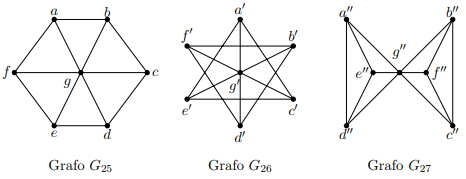
\includegraphics[width = 0.7\linewidth]{IsomorfismoEsercizio1}
		\end{figure}
	\end{center}
	\item
	Alcune condizioni necessarie:
	\begin{enumerate}
	\item
	$|\,V(G_{25})\,| = |\,V(G_{26})\,| = |\,V(G_{27})\,| = 7$ (\textsc{nulla si può dire})
	\item
	$|\,E(G)\,| = |\,E(G')\,| = |\,EV(G_{27})\,| = 12$ (\textsc{nulla si può dire})
	\item
	\textsc{Score:}
	\[
		\begin{rcases*}
		score(G_{25}) = (3,3,3,3,3,3,6) \\
		score(G_{25}) = (3,3,3,3,3,3,6) \\
		score(G_{25}) = (3,3,3,3,3,3,6)
		\end{rcases*} \textrm{\textsc{nulla si può dire}}
	\]
	\item
	$G_{25}$, $G_{26}$ e $G_{27}$ sono connessi.
	\item
	$G_{25}$ è $2\,$-connesso in quanto hamiltoniano, essendo $\{a,b,c,d,e,f,g,a\}$ un suo ciclo hamiltoniano.\\
	$G_{26}$ non è $2\,$-connesso in quanto $G_{26} - g'$ è un grafo con $2 \,c.c$ \\
	$G_{27}$ non è $2\,$-connesso in quanto $G_{27} - g''$ è un grafo con $2 \,c.c$ 
\begin{center}
	\begin{figure}[h!]
	  \centering
	  \begin{subfigure}[b]{0.3\linewidth}
	    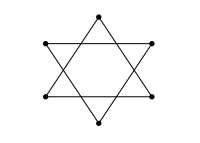
\includegraphics[width=\linewidth]{stella}
	    \caption{$G_{26} - g'$}
	  \end{subfigure}
	  \begin{subfigure}[b]{0.3\linewidth}
	    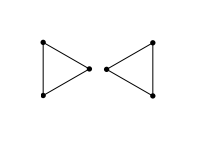
\includegraphics[width=\linewidth]{triangoli}
	    \caption{$G_{27} - g'$}
	  \end{subfigure}
	\end{figure}
\end{center}
	
	Dunque:
	$$G_{25} \not \simeq G_{26}$$
	$$G_{25} \not \simeq G_{27}$$
	\item
	$G_{26}$ e $G_{27}$ non sono $2\,$-connessi e dunque neanche hamiltoniani (\textsc{nulla si può dire}).
	\item
	Calcolare $\# (\{3,\dotso\,n\}$-cicli di $G)$ in generale è complicato e non porta a niente.
	\end{enumerate}
	\item
	Le costruzioni passano tutte le verifiche dunque \textsc{nulla si può dire}. Si passa a verifica diretta dell'isomorfismo tra $G_{26}$ e $G_{27}$:
	\begin{itemize}
	\item
	Costruiamo un isomorfimo $f: G_{26} \xrightarrow[\text{\quad\quad\quad}]{\text{}} G_{27}$
	\begin{equation}
	\begin{split}
	V_{26} & \xrightarrow[\text{\quad\quad\quad\quad\quad}]{\text{f}} V_{27} \\
		a' & \xmapsto[\text{\quad\,\quad\quad\quad\quad}]{\text{}} a'' \\
		b' & \xmapsto[\text{\quad\,\quad\quad\quad\quad}]{\text{}} b'' \\
		c' & \xmapsto[\text{\quad\,\quad\quad\quad\quad}]{\text{}} c'' \\
		d' & \xmapsto[\text{\quad\,\quad\quad\quad\quad}]{\text{}} d'' \\
		e' & \xmapsto[\text{\quad\,\quad\quad\quad\quad}]{\text{}} e'' \\
		f' & \xmapsto[\text{\quad\,\quad\quad\quad\quad}]{\text{}} f'' \\
		g' & \xmapsto[\text{\quad\,\quad\quad\quad\quad}]{\text{}} g''
		\notag
	\end{split}
	\end{equation}
	\item
	Osservo che $f$ è \textbf{iniettiva} (i vertici elencati nella colonna di destra sono a $2$ a $2$ distinti).
	\item
	Inoltre $f$ è \textbf{surgettiva} (nella colonna a destra compaiono tutti i vertici di $G_{27}$
	\item
	Dunque $f$ è una \textbf{bigezione}.
	\item
	Verifico se si tratta di un \textbf{morfismo} con $f^{-1}$ morfismo:
	\begin{equation}
	\begin{split}
	E(G_{26}) & \xrightarrow[\text{\quad\quad\quad\quad\quad}]{\text{'f'}} \displaystyle{\left(\frac{V(G_{27})}{2}\right)} \smallskip\smallskip \\	
		\{a',e' \} & \xmapsto[\text{\quad\,\quad\quad\quad\quad}]{\text{}} \{f'',c'' \} \quad \in E(G_{27}) \\
		\{a',g'\} & \xmapsto[\text{\quad\,\quad\quad\quad\quad}]{\text{}} \{f'',g''\} \quad \in E(G_{27}) \\		
		\{a',c'\} & \xmapsto[\text{\quad\,\quad\quad\quad\quad}]{\text{}} \{f'',b''\} \quad \in E(G_{27}) \\
		\{e',g'\} & \xmapsto[\text{\quad\,\quad\quad\quad\quad}]{\text{}} \{c'',g''\} \quad \in E(G_{27}) \\
		\{e',c'\} & \xmapsto[\text{\quad\,\quad\quad\quad\quad}]{\text{}} \{c'',b''\} \quad \in E(G_{27}) \\
		\{c',g'\} & \xmapsto[\text{\quad\,\quad\quad\quad\quad}]{\text{}} \{b'',g''\} \quad \in E(G_{27}) \\
		\{f',d'\} & \xmapsto[\text{\quad\,\quad\quad\quad\quad}]{\text{}} \{a'',d''\} \quad \in E(G_{27}) \\	
		\{f',b'\} & \xmapsto[\text{\quad\,\quad\quad\quad\quad}]{\text{}} \{a'',e''\} \quad \in E(G_{27}) \\
		\{f',g'\} & \xmapsto[\text{\quad\,\quad\quad\quad\quad}]{\text{}} \{e'',g''\} \quad \in E(G_{27}) \\
		\{b',d'\} & \xmapsto[\text{\quad\,\quad\quad\quad\quad}]{\text{}} \{e'',d''\} \quad \in E(G_{27}) \\
		\{b',g'\} & \xmapsto[\text{\quad\,\quad\quad\quad\quad}]{\text{}} \{e'',g''\} \quad \in E(G_{27}) \\
		\{d',g'\} & \xmapsto[\text{\quad\,\quad\quad\quad\quad}]{\text{}} \{d'',g''\} \quad \in E(G_{27})
		\notag
	\end{split}
	\end{equation}
	\item
	Se avessi trovato un lato che non appartiene a $E(G_{27})$ avrei dovuto rifare tutto, cambiando la funzione $f$ che ho definito in precedenza.
	\item
	Poichè i $2\,$-sottoinsiemi di $V(G_{27})$ che compaiono nella colonna di destra sono lati di $G_{27}$, segue che \textbf{$f$ è un morfismo}.
	\item
	Poichè nella colonna di destra compaiono tutti i lati di $G_{27}$, \textbf{$f$ è un isomorfismo}.
	\item
	In conclusione: $G_{26} \simeq G_{27}$
	\end{itemize}
	\end{itemize}
	
	\newpage
	\section{Score di grafi}
	\subsection{Esercizio 1}
	\begin{itemize}
	\item
	Dire se $d = (1,1,2,4,5,6,7)$ è lo score di un grafo.
	\begin{equation}
	\begin{split}
		n &= 7 \\
		d_n &= 7 \\ 
		& \\
		d_n \leq n - 1 &\Longleftrightarrow 7 \leq 7 - 1  \\
		&\Longleftrightarrow 7 \leq 6
		\notag
		\end{split}
	\end{equation}
	\item
	La prima ostruzione non è rispettata, dunque non esiste alcun grafo con score $d$.
	\end{itemize}
	
	\subsection{Esercizio 2}
	\begin{itemize}
	\item
	Dire se $d = (1,1,1,1,5,6,7,8)$ è lo score di un grafo.
	\begin{equation}
	\begin{split}
		n &= 8 \\
		d_n &= 8 \\ 
		& \\
		d_n \leq n - 1 &\Longleftrightarrow 8 \leq 8 - 1  \\
		&\Longleftrightarrow 8 \leq 7
		\notag
		\end{split}
	\end{equation}
	\item
	La prima ostruzione non è rispettata, dunque non esiste alcun grafo con score $d$.
	\end{itemize}
	
	\subsection{Esercizio 3}
	\begin{itemize}
	\item
	Dire se $d = (0,1,2,4,4,4,4,8,8,9)$ è lo score di un grafo.
	\item
	Supponiamo che esista un grafo finito $G$ con $score(G) = d$
	\item
	Allora $n := |V(G)| = 10$ e il grado massimo di uno dei suoi vertici è $d_n = 9$
	\item
	Deve valere:
	\begin{equation}
	\begin{split}
		d_n \leq n - 1 &\Longleftrightarrow 9 \leq 10 - 1  \\
		&\Longleftrightarrow 9 \leq 9
		\notag
		\end{split}
	\end{equation}
	\item
	La prima ostruzione è valida, \textbf{ma nulla si può dire}.
	\item
	Supponiamo che $d$ sia uno score di un grafo, allora anche $d' = (1,2,4,4,4,4,8,8,9)$ sarebbe lo score di un grado (quello precedente con il v\textbf{ertice isolato rimosso}).
	\item
	Allora vale:
	\begin{equation}
	\begin{split}
		d_n \leq n - 1 &\Longleftrightarrow 9 \leq 9 - 1  \\
		&\Longleftrightarrow 9 \leq 8
		\notag
		\end{split}
	\end{equation}
	\item
	La prima ostruzione non è rispettata, dunque non esiste alcun grafo con score $d'$, dunque neanche con $d$.
	\end{itemize}
	\subsection{Esercizio 4}
	\begin{itemize}
	\item
	Dire se $d = (1,1,2,2,2,3,4,5,5,7)$ è lo score di un grafo.
	\item
	Supponiamo che esista un grafo finito $G$ con $score(G) = d$
	\item
	Allora $n := |V(G)| = 10$ e il grado massimo di uno dei suoi vertici è $d_n = 7$
	\item
	Deve valere:
	\begin{equation}
	\begin{split}
		d_n \leq n - 1 &\Longleftrightarrow 7 \leq 10 - 1  \\
		&\Longleftrightarrow 7 \leq 9
		\notag
		\end{split}
	\end{equation}
	\item
	La prima ostruzione è valida, \textbf{ma nulla si può dire}.
	\item
	Per il lemma delle strette di mano, il numero di vertici dispari deve essere pari:
	\begin{equation}
	\begin{split}
		|&V(G) \textrm{ pari }| \quad\, =  4\\
		|&V(G) \textrm{ dispari }| = 3 
		\notag 
		\end{split}
	\end{equation}
	\item
	Il lemma delle strette di mano (ostruzione $n.2$) non è rispettato, dunque non esiste alcun grafo con score $d$.
	\end{itemize}
	
	\subsection{Esercizio 5}
	\begin{itemize}
	\item
	Dire se $d = (1,2,3,4,5,6,7,8,8)$ è lo score di un grafo.
	\item
	Supponiamo che esista un grafo finito $G$ con $score(G) = d$
	\item
	Allora $n := |V(G)| = 9$ e il grado massimo di uno dei suoi vertici è $d_n = 8$
	\item
	Deve valere:
	\begin{equation}
	\begin{split}
		d_n \leq n - 1 &\Longleftrightarrow 8 \leq 9 - 1  \\
		&\Longleftrightarrow 8 \leq 8
		\notag
		\end{split}
	\end{equation}
	\item
	La prima ostruzione è valida, \textbf{ma nulla si può dire}.
	\item
	Per il lemma delle strette di mano, il numero di vertici dispari deve essere pari:
	\begin{equation}
	\begin{split}
		|&V(G) \textrm{ pari }| \quad\, =  4\\
		|&V(G) \textrm{ dispari }| = 4 
		\notag
		\end{split}
	\end{equation}
	\item
	La seconda ostruzione è rispettata, \textbf{ma nulla si può dire}.
	\item
	Siamo nelle ipotesi della terza ostruzione, cioè lo score termina con termini che valgono $n-1$, ma deve valere anche $k < d_1$, cioè il numero di termini che valgono $n-1$ deve essere minore del primo termine dello score.
	\item
	Vale:
	\begin{equation}
	\begin{split}
		k &< d_1 \\
		2 &< 1
		\notag
		\end{split}
	\end{equation}
	\item
	La terza ostruzione non è rispettata, dunque non esiste alcun grafo con score $d$.
	\end{itemize}
	
	\subsection{Esercizio 6}
	\begin{itemize}
	\item
	Dire se $d = (2,2,3,3,3,3,4,4,11,11,11)$ è lo score di un grafo.
	\item
	Supponiamo che esista un grafo finito $G$ con $score(G) = d$
	\item
	Allora $n := |V(G)| = 12$ e il grado massimo di uno dei suoi vertici è $d_n = 11$
	\item
	Deve valere:
	\begin{equation}
	\begin{split}
		d_n \leq n - 1 &\Longleftrightarrow 11 \leq 12 - 1  \\
		&\Longleftrightarrow 11 \leq 11
		\notag
		\end{split}
	\end{equation}
	\item
	La prima ostruzione è valida, \textbf{ma nulla si può dire}.
	\item
	Per il lemma delle strette di mano, il numero di vertici dispari deve essere pari:
	\begin{equation}
	\begin{split}
		|&V(G) \textrm{ pari }| \quad\, =  4\\
		|&V(G) \textrm{ dispari }| = 8 
		\notag
		\end{split}
	\end{equation}
	\item
	La seconda ostruzione è rispettata, \textbf{ma nulla si può dire}.
	\item
	Siamo nelle ipotesi della terza ostruzione, cioè lo score termina con termini che valgono $n-1$, ma deve vale anche $k < d_1$, cioè il numero di termini che valgono $n-1$ deve essere minore del primo termine dello score.
	\item
	Vale:
	\begin{equation}
	\begin{split}
		k &< d_1 \\
		3 &< 2
		\notag
		\end{split}
	\end{equation}
	\item
	La terza ostruzione non è rispettata, dunque non esiste alcun grafo con score $d$.
	\end{itemize}
	
	\subsection{Esercizio 7}
	\begin{itemize}
	\item
	Dire se $d = (1,1,2,2,2,2,2,2,2,3,4,4,12,13)$ è lo score di un grafo.
	\item
	Supponiamo che esista un grafo finito $G$ con $score(G) = d$
	\item
	Allora $n := |V(G)| = 14$ e il grado massimo di uno dei suoi vertici è $d_n = 13$
	\item
	Deve valere:
	\begin{equation}
	\begin{split}
		d_n \leq n - 1 &\Longleftrightarrow 13 \leq 14 - 1  \\
		&\Longleftrightarrow 13 \leq 13
		\notag
		\end{split}
	\end{equation}
	\item
	La prima ostruzione è valida, \textbf{ma nulla si può dire}.
	\item
	Per il lemma delle strette di mano, il numero di vertici dispari deve essere pari:
	\begin{equation}
	\begin{split}
		|&V(G) \textrm{ pari }| \quad\, =  10\\
		|&V(G) \textrm{ dispari }| = 4 
		\notag
		\end{split}
	\end{equation}
	\item
	La seconda ostruzione è rispettata, \textbf{ma nulla si può dire}.
	\item
	Non siamo nelle ipotesi della terza ostruzione, perchè lo score termina con un solo termine che vale $n-1$, dunque visto che "ex falso quodlibet", cioè "dal falso segue qualsiasi cosa", la terza ostruzione è rispettata.
	\item
	Verifichiamo la quarta ostruzione, cioè "il numero di entrate di $d$ (eccetto le ultime due) maggiori o uguali a $2$" deve essere maggiore di $d_{n-1} + d_n - n$
	\item
	Dunque:
	\begin{equation}
	\begin{split}
		|(2,2,2,2,2,2,2,3,4,4,12,13)| &\geq 12+13-14 \\
		10 &\geq 11
		\notag
		\end{split}
	\end{equation}
	\item
	La quarta ostruzione non è rispettata, dunque non esiste alcun grafo con score $d$.
	\end{itemize}
	
	\newpage
	\section{Teorema dello score}
	\subsection{Enunciato}
	\begin{itemize}
	\item
	Sia $n \geq 2$ e sia $d = (d_1, d_2, \dotso\,,d_n) \in \mathbb{N}^n$ tale che $0 \leq d_1 \leq \dotso \leq d_n \leq n-1$
	\item
	Definiamo il seguente vettore $d' = (d^{'}_1, d^{'}_2, \dotso\,,d^{'}_{n-1}) \in \mathbb{N}^{n-1}$
	\begin{equation}
	d_{i}' := 
	\begin{cases}
	d_i & i < n-d_n \\
	d_i - 1 & i \geq n-d_n
	\end{cases}
	\end{equation}
	\item
	Allora $d$ è lo score di un grafo se e soltanto se lo è $d'$.
	\item
	Se tutto degenera e va a 0, allora $d'$ è lo score di un grafo, e di conseguenza anche $d$ è lo score di un grafo.
	\item
	Per semplicità nei calcoli, quando le entrate dell' i-esimo score sono tutte minori o uguali a $2$ ci si può fermare.
	\end{itemize}
	\subsection{Esercizio 1}
	\begin{itemize}
	\item
	Dire se $d = (2,2,3,3,3,3,4,4,11,11,11)$ è lo score di un grafo.
	\item
	Supponiamo che esista un grafo finito $G$ con $score(G) = d$
	\item
	Allora $n := |V(G)| = 12$ e il grado massimo di uno dei suoi vertici è $d_n = 11$
	\item
	Deve valere:
	\begin{equation}
	\begin{split}
		d_n \leq n - 1 &\Longleftrightarrow 11 \leq 12 - 1  \\
		&\Longleftrightarrow 11 \leq 11
		\notag
		\end{split}
	\end{equation}
	\item
	La prima ostruzione è valida, \textbf{ma nulla si può dire}.
	\item
	Per il lemma delle strette di mano, il numero di vertici dispari deve essere pari:
	\begin{equation}
	\begin{split}
		|&V(G) \textrm{ pari }| \quad\, =  4\\
		|&V(G) \textrm{ dispari }| = 8 
		\notag
		\end{split}
	\end{equation}
	\item
	La seconda ostruzione è rispettata, \textbf{ma nulla si può dire}.
	\item
	Siamo nelle ipotesi della terza ostruzione, cioè lo score termina con termini che valgono $n-1$, ma deve valere anche $k < d_1$, cioè il numero di termini che valgono $n-1$ deve essere minore del primo termine dello score.
	\item
	Vale:
	\begin{equation}
	\begin{split}
		k &< d_1 \\
		3 &< 2
		\notag
		\end{split}
	\end{equation}
	\item
	La terza ostruzione non è rispettata, dunque non esiste alcun grafo con score $d$.
	\end{itemize}
	
	\subsection{Esercizio 2}
	\begin{itemize}
	\item
	Dire se $d = (2,2,2,2,3,3,5,5,8,8)$ è lo score di un grafo.
	\item
	Supponiamo che esista un grafo finito $G$ con $score(G) = d$
	\item
	Allora $n := |V(G)| = 10$ e il grado massimo di uno dei suoi vertici è $d_n = 8$
	\item
	Deve valere:
	\begin{equation}
	\begin{split}
		d_n \leq n - 1 &\Longleftrightarrow 8 \leq 10 - 1  \\
		&\Longleftrightarrow 8 \leq 9
		\notag
		\end{split}
	\end{equation}
	\item
	La prima ostruzione è valida, \textbf{ma nulla si può dire}.
	\item
	Per il lemma delle strette di mano, il numero di vertici dispari deve essere pari:
	\begin{equation}
	\begin{split}
		|&V(G) \textrm{ pari }| \quad\, =  6\\
		|&V(G) \textrm{ dispari }| = 4 
		\notag
		\end{split}
	\end{equation}
	\item
	La seconda ostruzione è rispettata, \textbf{ma nulla si può dire}.
	\item
	La terza ostruzione è verificata.
	\item
	Verifichiamo la quarta ostruzione, cioè "il numero di entrate di $d$ (eccetto le ultime due) maggiori o uguali a $2$" deve essere maggiore di $d_{n-1} + d_n - n$
	\item
	Dunque:
	\begin{equation}
	\begin{split}
		|(2,2,2,2,3,3,5,5,8,8)| &\geq 8+8-10 \\
		8 &\geq 6
		\notag
		\end{split}
	\end{equation}
	\item
	La quarta ostruzione è rispettata, \textbf{ma nulla si può dire}.
	\item
	Le ostruzioni non forniscono informazioni, applico quindi il \textbf{teorema dello score}:
	\[
	\begin{array}{cc}
		\toprule
		Score & Dati \\
		\midrule
		\begin{split} d &= (2,2,2,2,3,3,5,5,8,8) \end{split} & \begin{split} n &= 10 \\ d_n &= 8 \leq 10 -1 \end{split} \\
		\midrule
		\begin{split} d' &= (2,1,1,1,2,2,4,4,7) \\ &= (1,1,1,2,2,2,4,4,7) \end{split} & \begin{split} n &= 9 \\ d_n &= 7 \leq 9 -1 \end{split} \\
		\midrule
		\begin{split} d'' &= (1,0,0,1,1,1,3,3) \\ &= (0,0,1,1,1,1,3,3) \end{split} & \begin{split} n &= 8 \\ d_n &= 3 \leq 8 -1 \end{split} \\
		\midrule
		\begin{split} d''' &= (0,0,1,1,0,0,2) \\ &= (0,0,0,0,1,1,2)  \end{split} & \textrm{Entrate minori o uguali a 2} \\
		\bottomrule
	\end{array}
	\]
	\item
	Poichè $d'''$ è lo score del seguente grafo $G'''$:
	\begin{center}
		\begin{figure}[h]
		\centering
		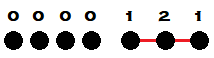
\includegraphics[width = 0.2\linewidth]{scoreGrafo_Esercizio2}
	\end{figure}
	\end{center}
	\item
	Dunque, grazie al teorema dello score anche $d$ è lo score di un grafo G.
	\end{itemize}
	
	\subsection{Esercizio 3}
	\begin{itemize}
	\item
	Dire se $d = (2,2,2,2,3,3,5,6)$ è lo score di un grafo.
	\item
	Supponiamo che esista un grafo finito $G$ con $score(G) = d$
	\item
	Allora $n := |V(G)| = 9$ e il grado massimo di uno dei suoi vertici è $d_n = 6$
	\item
	Deve valere:
	\begin{equation}
	\begin{split}
		d_n \leq n - 1 &\Longleftrightarrow 6 \leq 9 - 1  \\
		&\Longleftrightarrow 6 \leq 8
		\notag
		\end{split}
	\end{equation}
	\item
	La prima ostruzione è valida, \textbf{ma nulla si può dire}.
	\item
	Per il lemma delle strette di mano, il numero di vertici dispari deve essere pari:
	\begin{equation}
	\begin{split}
		|&V(G) \textrm{ pari }| \quad\, =  5\\
		|&V(G) \textrm{ dispari }| = 4 
		\notag
		\end{split}
	\end{equation}
	\item
	La seconda ostruzione è rispettata, \textbf{ma nulla si può dire}.
	\item
	La terza ostruzione è verificata, in quanto lo score termina con $6$ e non con $n-1 = 9 -1 = 8$
	\item
	Verifichiamo la quarta ostruzione, cioè "il numero di entrate di $d$ (eccetto le ultime due) maggiori o uguali a $2$" deve essere maggiore di $d_{n-1} + d_n - n$
	\item
	Dunque:
	\begin{equation}
	\begin{split}
		|(2,2,2,2,3,3,5,6)| &\geq 5+6-9 \\
		7 &\geq 2
		\notag
		\end{split}
	\end{equation}
	\item
	La quarta ostruzione è rispettata, \textbf{ma nulla si può dire}.
	\item
	Le ostruzioni non forniscono informazioni, applico quindi il \textbf{teorema dello score}:
	\[
	\begin{array}{cc}
		\toprule
		Score & Dati \\
		\midrule
		\begin{split} d &= (2,2,2,2,3,3,5,6) \end{split} & \begin{split} n &= 9 \\ d_n &= 6 \leq 9 -1 \end{split} \\
		\midrule
		\begin{split} d' &= (2,2,1,1,2,2,2,4) \\ &= (1,1,2,2,2,2,2,4) \end{split} & \begin{split} n &= 8 \\ d_n &= 4 \leq 8 -1 \end{split} \\
		\midrule
		\begin{split} d'' &= (1,1,2,1,1,1,1) \\ &= (1,1,1,1,1,1,2) \end{split} & \textrm{Entrate minori o uguali a 2} \\
		\bottomrule
	\end{array}
	\]
	\item
	Poichè $d'''$ è lo score del seguente grafo $G'''$:
	\begin{center}
		\begin{figure}[h]
		\centering
		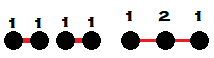
\includegraphics[width = 0.2\linewidth]{scoreGrafo_Esercizio3}
	\end{figure}
	\end{center}
	\item 
	Dunque, grazie al teorema dello score anche $d$ è lo score di un grafo G.
	\item
	Costruiamo un grafo (procedura a ritroso) con score $d$ utilizzando il teorema dello score:
	\end{itemize}
	
	\subsection{Esercizio 4}
	\begin{itemize}
	\item
	Dire se $d = (3,3,3,3,4,4,4,4,4,4,13,13,13,13)$ è lo score di un grafo.
	\item
	Supponiamo che esista un grafo finito $G$ con $score(G) = d$
	\item
	Allora $n := |V(G)| = 14$ e il grado massimo di uno dei suoi vertici è $d_n = 13$
	\item
	Deve valere:
	\begin{equation}
	\begin{split}
		d_n \leq n - 1 &\Longleftrightarrow 13 \leq 14 - 1  \\
		&\Longleftrightarrow 13 \leq 13
		\notag
		\end{split}
	\end{equation}
	\item
	La prima ostruzione è valida, \textbf{ma nulla si può dire}.
	\item
	Per il lemma delle strette di mano, il numero di vertici dispari deve essere pari:
	\begin{equation}
	\begin{split}
		|&V(G) \textrm{ pari }| \quad\, =  6\\
		|&V(G) \textrm{ dispari }| = 8 
		\notag
		\end{split}
	\end{equation}
	\item
	La seconda ostruzione è rispettata, \textbf{ma nulla si può dire}.
	\item
	Se $d$ fosse lo score di un grado, per la terza ostruzione sarebbero previsti $4$ vertici di grado $13 = n-1$ (dove $n=14$ è il numero di vertici) che dovrebbero essere collegati a tutti gli altri vertici.
	\item
	Dunque il grado minimo previsto dovrebbe essere maggiore o uguale a $4$, che è assurdo visto che il grado minimo dello score $d$ è $3$.
	\item
	La terza ostruzione non è rispettata, dunque non esiste un grafo con score d.
	\end{itemize}	
	
	\subsection{Esercizio 5}
	\begin{itemize}
	\item
	Dire se $d = (1,1,1,1,1,1,1,1,1,1,4,4,4)$
	\item
	Supponiamo che esista un grafo finito $G$ con $score(G) = d$
	\item
	Allora $n := |V(G)| = 13$ e il grado massimo di uno dei suoi vertici è $d_n = 4$
	\item
	Deve valere:
	\begin{equation}
	\begin{split}
		d_n \leq n - 1 &\Longleftrightarrow 4 \leq 13 - 1  \\
		&\Longleftrightarrow 4 \leq 12
		\notag
		\end{split}
	\end{equation}
	\item
	La prima ostruzione è valida, \textbf{ma nulla si può dire}.
	\item
	Per il lemma delle strette di mano, il numero di vertici dispari deve essere pari:
	\begin{equation}
	\begin{split}
		|&V(G) \textrm{ pari }| \quad\, =  3\\
		|&V(G) \textrm{ dispari }| = 10 
		\notag
		\end{split}
	\end{equation}
	\item
	La seconda ostruzione è rispettata, \textbf{ma nulla si può dire}.
	\item
	La terza ostruzione è verificata, in quanto non è possibile controllarla.
	\item
	Verifichiamo la quarta ostruzione, cioè "il numero di entrate di $d$ (eccetto le ultime due) maggiori o uguali a $2$" deve essere maggiore di $d_{n-1} + d_n - n$
	\item
	Dunque:
	\begin{equation}
	\begin{split}
		|(1,1,1,1,1,1,1,1,1,1,4,4,4)| &\geq 4+4-13 \\
		1 &\geq -5
		\notag
		\end{split}
	\end{equation}
	\item
	La quarta ostruzione è rispettata, \textbf{ma nulla si può dire}.
	\item
	Le ostruzioni non forniscono informazioni, applico quindi il \textbf{teorema dello score} a $d_2$:
	\[
	\begin{array}{cc}
		\toprule
		Score & Dati \\
		\midrule
		\begin{split} d &= (1,1,1,1,1,1,1,1,1,1,4,4,4) \end{split} & \begin{split} n &= 13 \\ d_n &= 4 \leq 13 -1 \end{split} \\
		\midrule
		\begin{split} d' &= (1,1,1,1,1,1,1,1,0,0,3,3) \\ &= (0,0,1,1,1,1,1,1,1,1,3,3) \end{split} & \begin{split} n &= 12 \\ d_n &= 3 \leq 12 -1 \end{split} \\
		\midrule
		\begin{split} d'' &= (0,0,1,1,1,1,1,0,0,2) \\ &= (0,0,0,0,1,1,1,1,1,1,2) \end{split} & \textrm{Entrate minori o uguali a 2} \\
		\bottomrule
	\end{array}
	\]
	\item
	Poichè $d''$ è lo score del seguente grafo $G'''$:
	\begin{center}
		\begin{figure}[h]
		\centering
		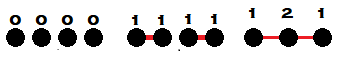
\includegraphics[width = 0.2\linewidth]{scoreGrafo_Esercizio5}
	\end{figure}
	\end{center}
	\item 
	Grazie al teorema dello score anche $d_2$ è lo score di un grafo $G_2$.
	\item
	Costruiamo un grafo (procedura a ritroso) con score $d$ utilizzando il teorema dello score:
	\begin{center}
		\begin{figure}[h]
		\centering
		\begin{subfigure}[b]{0.4\linewidth}
			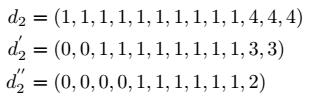
\includegraphics[width=\linewidth]{scoreEsercizio5}
		\end{subfigure}
		\begin{subfigure}[b]{0.2\linewidth}
			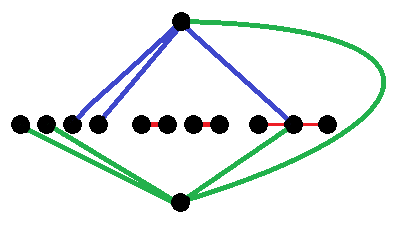
\includegraphics[width=\linewidth]{grafoEsercizio5}
		\end{subfigure}
	\end{figure}
	\end{center}
	\end{itemize}
\end{document} 